
% vim: set ts=4 sw=4 tw=80 noexpandtab:
%******************************************************************************%
%                                                                              %
%                   Vogsphere.tex                                              %
%                   Made by: 42 staff                                          %
%                                                                              %
%******************************************************************************%

\documentclass{42-en}

%******************************************************************************%
%                                                                              %
%                                   Prologue                                   %
%                                                                              %
%******************************************************************************%

\begin{document}

\title{Vogsphere, Github, \& Bitbucket Cheat Sheet}
\subtitle{Is This Thing On?}

\member {Kai}{kai@42.us.org}

\summary
{
With greatly confusing commands comes great collaboration ability.
}

\maketitle

\tableofcontents

%Initialisation des headers d'exercices

\startexercices


%******************************************************************************%
%                                                                              %
%                                    Preamble                                  %
%                                                                              %
%******************************************************************************%

\chapter{Preamble}

\begin{figure}[H]
    \begin{center}
        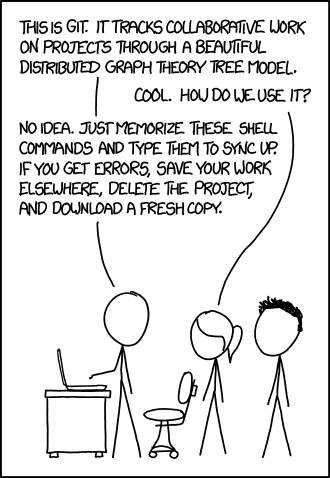
\includegraphics[width=8cm]{images/xkcd_git.png}
    \end{center}
\end{figure}

Read about our love-hate relationship with git at \texttt{\href{https://explainxkcd.com/wiki/index.php/1597:_Git}{explainxkcd.com}}.\\

\noindent Beginner-friendly reference at \href{http://gitready.com/}{git ready}!

%******************************************************************************%
%                                                                              %
%                                   Clone                                      %
%                                                                              %
%******************************************************************************%

\chapter{Clone your Repository}

Recommended reference \& optional effort: Michael Hartl's \href{https://www.learnenough.com/git-tutorial}{"Learn Enough Git to be Dangerous"}.

\begin{enumerate}

\item From your \href{https://projects.intra.42.fr/h2s-first-day/mine}{First Day project page} on intra, copy the "Git Repository" link. (The one that looks like vogsphere@vgs.42.us.org:intra/2017...). If you do not have a link yet, make sure you are registered to the project, and wait about 5 minutes while refreshing the page.

\item Your Vosphere respositories have permissions connected to them which control who can download or add to the responsitory. In order to identify yourself from the terminal, type \texttt{"kinit <username>"} and press enter. Next, type your 42 password and press enter.

\item Now, in the terminal type \texttt{"git clone <copied link> (space) <newfoldername>"}. Replace <link> with your pasted link and <newfoldername> with a relevant name for the project folder. Press Enter.

\item \texttt{cd <foldername>} to move into the newly created folder. Everything that you place inside here can be uploaded to Vogsphere. You can also move files into this folder using Finder or the \texttt{"cp" (copy)} and \texttt{"mv" (move)} commands.

\item Complete the project requirements (see next page). All files for the project should go in the folder we just created.

\end{enumerate}

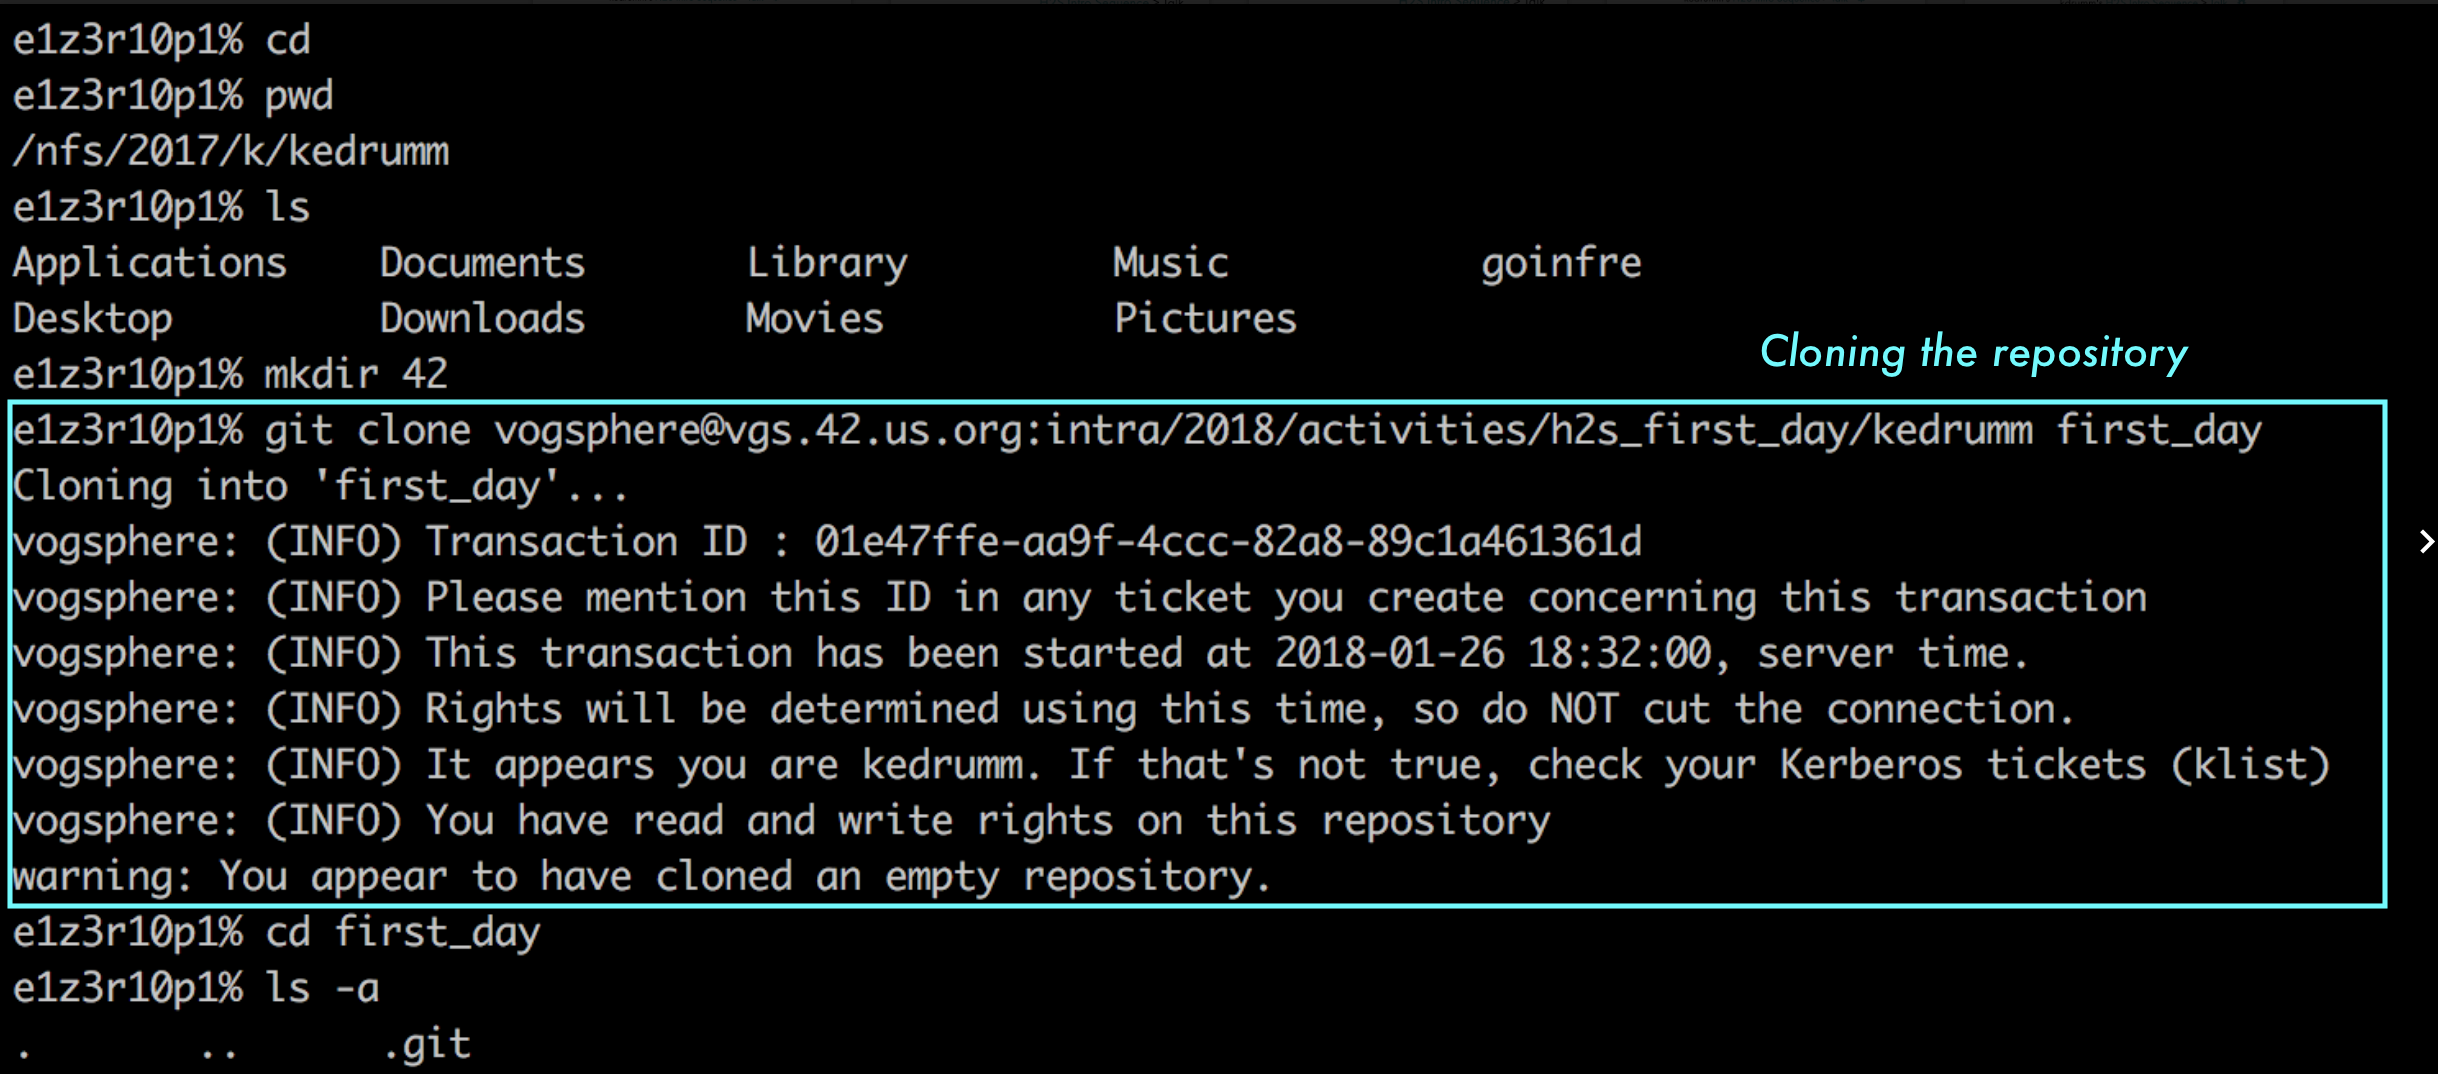
\includegraphics[width=1\textwidth]{screenshots/clone_first_day}

%******************************************************************************%
%                                                                              %
%                               Turning In Your Code                           %
%                                                                              %
%******************************************************************************%

\chapter{Turning in your code}

Turn in your work by typing three commands in order (and press enter after each one):
	\begin{itemize}
		\item \texttt{git add *}
		\item \texttt{git commit -m "Today I worked on ..<your comments here>.."}
		\item \texttt{git push}
	\end{itemize}
	\hint{Make sure you are in your project's git folder when you type the git add, git commit, git push commands.}
	\hint{If you have an error during the git push, you may need to refresh your authentication ticket. Do this by typing "kinit <username>" and then typing your intra password.}

Back on Intra, you can press the button "Set the Project as Finished" to indicate that you are ready for corrections.

	\hint{Pushing to Vogsphere more often is one way of saving your work.}


%******************************************************************************%
%                                                                              %
%                                   Git Tips                                   %
%                                                                              %
%******************************************************************************%

\chapter{Git Tips}

\begin{enumerate}
	
	\item You can tell that you are inside the correct folder for turning in your projects in a couple of ways. First of all, you can tell it's a git folder by typing \texttt{"ls -a"} and pressing enter. You will see the hidden .git folder which contains the files that git uses to keep track of changes.

	\item Type \texttt{"git remote -v"} and enter. This will tell you what \texttt{remote branches} your git folder is connected to. By default, they should be the Vogsphere link that you copied earlier. If you read some git tutorials and/or talk to your mentor, you can set this up to connect to your personal Github or Bitbucket repositories as well.

	\item Type \texttt{"git log"} and enter. This shows a history of changes you have made to your git repository.

	\item To help with committing and pushing, type \texttt{"git status"}. It will tell you which files have been \texttt{added} to git and which ones have been \texttt{pushed}.

\end{enumerate}

%******************************************************************************%
%                                                                              %
%                                 Corrections                                  %
%                                                                              %
%******************************************************************************%

\chapter{Corrections}
\begin{itemize}
	\item On your project page, click the button "Subscribe to Defense." Choose a time slot from the screen that shows next.

	\item When the appointment time comes, look up your assigned corrector on Slack or Discord and send them a message. Find each other.

	\item Corrector, sit at the correctee's station and open a new web browser in Incognito mode. Log into your intra.

	\item Access the corrections page. Clone their Git repository into a new folder.

	\item Click "Begin correction" and follow the instructions on the correction page.

	\item Discuss the code and feel free to chat about life.

	\item Once the correction is finished, your corrector should remember to log out of Intra.

	\item After both the correction is complete, in order to finalize your score you must then provide feedback for the corrector on your project page. Go to your project page and click the "feedback" button for each completed correction.

\end{itemize}

%******************************************************************************%
%                                                                              %
%                               End of document                                %
%                                                                              %
%******************************************************************************%

\end{document}

